\begin{figure}[b]
\begin{center}
	\resizebox{0.4\textwidth}{!}{%
 		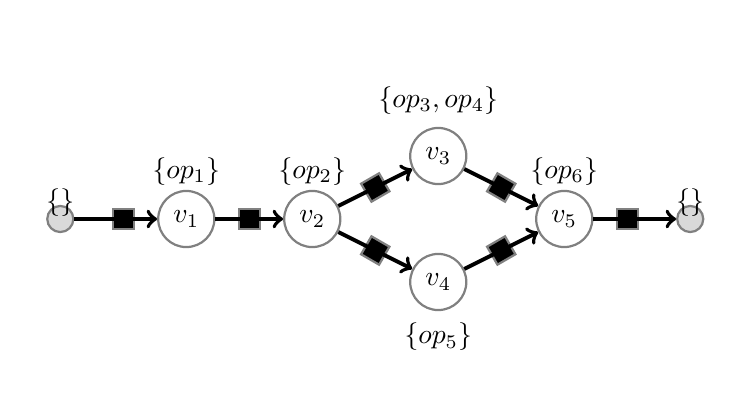
\begin{tikzpicture} 
 %[scale=.8,auto=left,every node/.style={circle,fill=blue!20}]
             [scale=.8,auto=left,every node/.style={circle,draw=black!50, thick},every path/.style={line width=0.5mm}]
 			\node[circle, fill=gray!30,label={[xshift=0cm, yshift=-0.4cm]$\{\optop\}$}] (v_t) at (-5,0) {$\verttop$};
             \node[label={[xshift=0cm, yshift=-0.4cm]$\{op_1\}$}] (v_1) at (-3,0) {$v_1$};
             \node[label={[xshift=0cm, yshift=-0.4cm]$\{op_2\}$}] (v_2) at (-1,0) {$v_2$};
             \node[label={[xshift=0cm, yshift=-0.6cm]$\{op_3,op_4\}$}] (v_3) at (1,1) {$v_3$};
             \node[label={[xshift=0cm, yshift=-1.7cm]$\{op_5\}$}] (v_4) at (1,-1) {$v_4$};
             \node[label={[xshift=0cm, yshift=-0.4cm]$\{op_6\}$}] (v_5) at (3,0) {$v_5$};                         
 			\node[circle, fill=gray!30,label={[xshift=0cm, yshift=-0.4cm]$\{\opbot\}$}] (v_b) at (5,0) {$\vertbot$};
			
			\node[rectangle,fill=black,minimum size=7.5pt] (v_c) at (-4,0) {};			
			\node[rectangle,fill=black,minimum size=7.5pt] (v_c) at (-2,0) {};
			\node[rectangle,fill=black,minimum size=7.5pt,rotate=30] (v_c) at (0,0.5) {};             
			\node[rectangle,fill=black,minimum size=7.5pt,rotate=60] (v_c) at (0,-0.5) {};          
			\node[rectangle,fill=black,minimum size=7.5pt,rotate=60] (v_c) at (2,0.5) {};  
			\node[rectangle,fill=black,minimum size=7.5pt,rotate=30] (v_c) at (2,-0.5) {}; 
			\node[rectangle,fill=black,minimum size=7.5pt] (v_c) at (4,0) {}; 	
			\node[rectangle,fill=black,minimum size=7.5pt] (v_c) at (-2,0) {};  		
			
 			\path[line width=0.5mm] (v_t) edge[->] (v_1);
 			\path (v_1) edge[->] (v_2);
 			\path (v_2) edge[->] (v_3);
 			\path (v_2) edge[->] (v_4); 
 			\path (v_3) edge[->] (v_5); 						
 			\path (v_4) edge[->] (v_5);
 			\path (v_5) edge[->] (v_b);
 		\end{tikzpicture}
 	}
 	\end{center}
\caption{The plant graph of the linear model case.}
\label{fig:linear_plant_graph}
\end{figure}


\begin{figure*}[!t]
\centering
    \begin{subfigure}[t]{0.33\linewidth}
        \centering
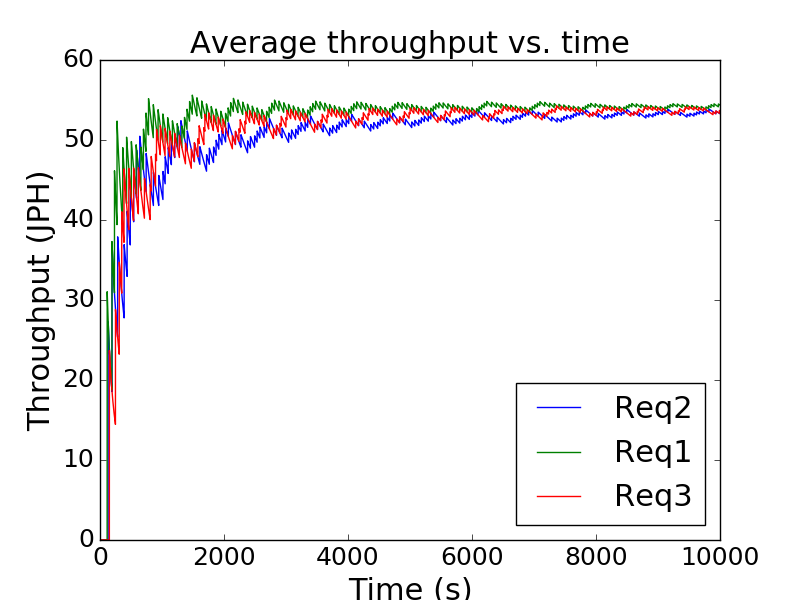
\includegraphics[width=0.99\columnwidth]{Figures/b2-throughput}
%\vspace{-\baselineskip}
\caption{Throughput of each widget (JPH).}
\label{fig:linear_jph}
%\vspace{-1\baselineskip}
    \end{subfigure}%
        ~%\hspace{0.5cm} 
    \begin{subfigure}[t]{0.33\linewidth}
        \centering     
        %\vspace{3\baselineskip}     
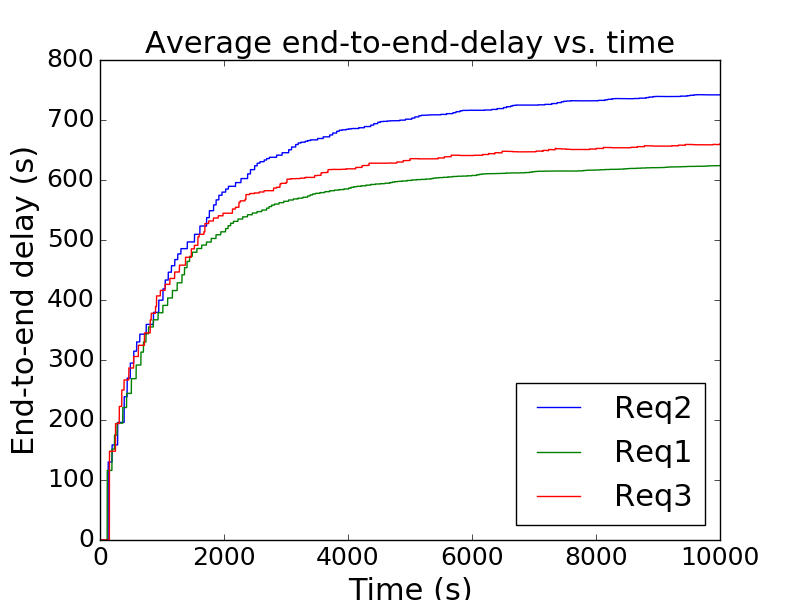
\includegraphics[width=0.99\columnwidth]{Figures/b2-end-to-end}
%\vspace{-\baselineskip}
\caption{End-to-end time of each widget.}
\label{fig:linear_end_to_end}
    \end{subfigure}%
        ~ 
    \begin{subfigure}[t]{0.33\linewidth}
        \centering     
 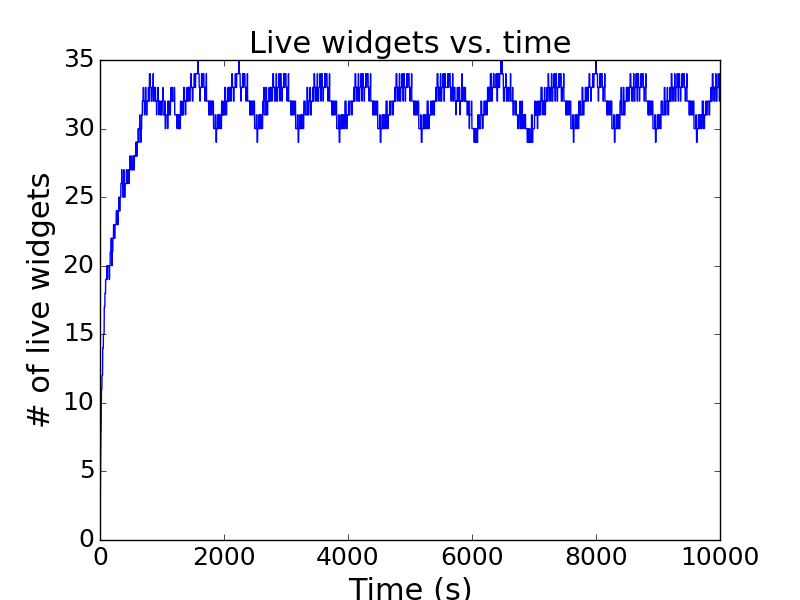
\includegraphics[width=0.99\columnwidth]{Figures/b2-total-widgets}
%\vspace{-\baselineskip}
\caption{Total alive widgets in the plant.}
\label{fig:linear_total_widgets}
        %\vspace{-\baselineskip}
    \end{subfigure}
    %\vspace{-\baselineskip}
    \caption{Experiment results for the plant shown in Figure~\ref{fig:linear_plant_graph}.}
    \label{fig:linear_model_exp}
    %\vspace{-1\baselineskip}
\end{figure*}



\begin{figure*}[!t]
\centering
    \begin{subfigure}[t]{0.33\linewidth}
        \centering
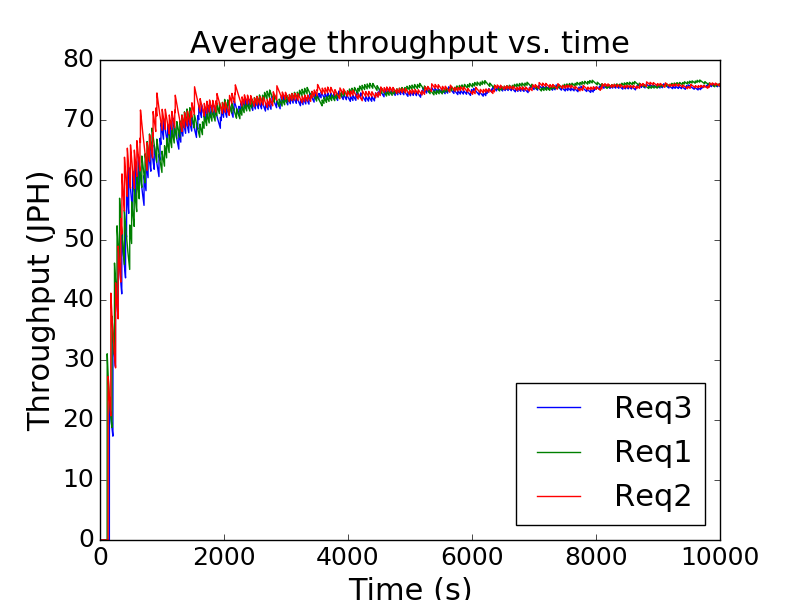
\includegraphics[width=0.99\columnwidth]{Figures/b3-throughput}
%\vspace{-\baselineskip}
\caption{Throughput of each widget (JPH).}
\label{fig:linear_plus_jph}
%\vspace{-1\baselineskip}
    \end{subfigure}%
        ~%\hspace{0.5cm} 
    \begin{subfigure}[t]{0.33\linewidth}
        \centering     
        %\vspace{3\baselineskip}     
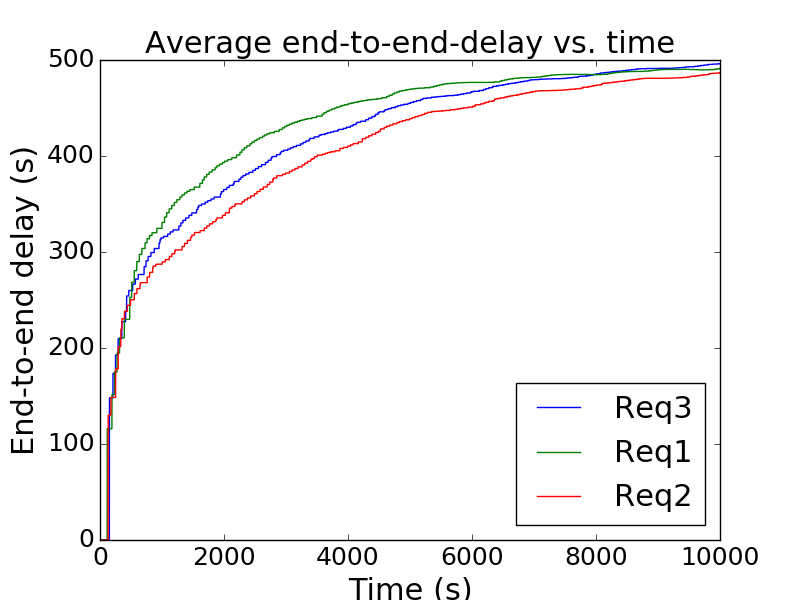
\includegraphics[width=0.99\columnwidth]{Figures/b3-end-to-end}
%\vspace{-\baselineskip}
\caption{End-to-end time of each widget.}
\label{fig:linear_plus_end_to_end}
    \end{subfigure}%
        ~ 
    \begin{subfigure}[t]{0.33\linewidth}
        \centering     
 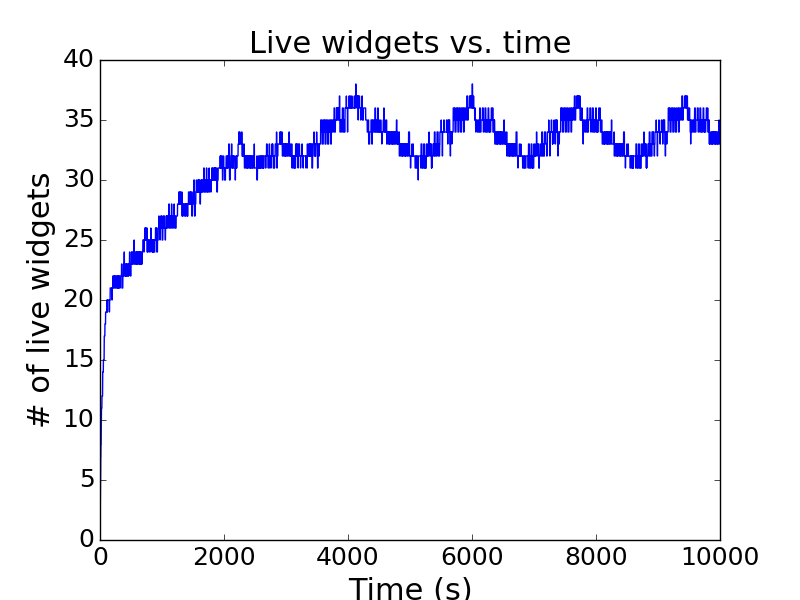
\includegraphics[width=0.99\columnwidth]{Figures/b3-total-widgets}
%\vspace{-\baselineskip}
\caption{Total alive widgets in the plant.}
\label{fig:linear_plus_total_widgets}
        %\vspace{-\baselineskip}
    \end{subfigure}
    %\vspace{-\baselineskip}
    \caption{Experiment results for the plant that has an additional cell, $v_6$, as shown in Figure~\ref{fig:linear_plant_plus_graph}.}
    \label{fig:linear_plus_exp}
    %\vspace{-1\baselineskip}
\end{figure*}

\section{Case Study}
\label{sec:case_study}
In this section we use a synthetic linear model and its variant as examples to demonstrate the use of the \mfname modeling framework.
We also carry out analysis using the simulator described in Section~\ref{sec:simulation}.

\subsection{A Synthetic Linear Model}
\label{subsec:linear_model}
Let's consider a simple linear manufacturing system consisting of five cells, $V=\{v_1,v_2,v_3,v_4,v_5\}$.
This plant contains a fork that provides multiple path options for dynamic allocation and support for fabricating multiple types of widgets.
The plant is represented as a graph (Figure~\ref{fig:linear_plant_graph}).
The supported operations and the time for each node to complete the designated operation is:\\

\begingroup
\setlength\parindent{24pt}
\indent $v_1 \colon \ T(v_1,op_1)=10s$\\
\indent $v_2 \colon \ T(v_2,op_2)=20s$\\
\indent $v_3 \colon \ T(v_3,op_3)=40s,\ T(v_3,op_4)=35s$\\
\indent $v_4 \colon \ T(v_4,op_5)=50s$\\
\indent $v_5 \colon \ T(v_5,op_6)=15s$\\
\endgroup





Let's consider three types of widgets to be fabricated in this plant, denoted by $\mathcal{R}=\{R_1,R_2,R_3\}$.
These requirements are listed in Table~\ref{tab:linear_plant_requirements}.
Requirement 1 is a typical linear manufacturing process that requires the widgets to visit the cells that support the corresponding operations in the given order.
Requirement 2 shows a different set of operations potentially requiring some cells to be bypassed.
For example, the path satisfying $R_2$ in the given plant is $\verttop \ra v_1 \ra v_2 \ra v_4 \ra v_5 \ra \vertbot$ where $v_1$ and $v_5$ do nothing to the widgets under this requirement.
Requirement 3 has an option for the system to choose a path that satisfies one of the operation requirements (\ie either $op_4$ or $op_5$ at the second stage).
These types of requirements are not uncommon since different models of machines can perform the same work on the widgets albeit with different tools.

\begin{table}[t]
\centering
\caption{Operational requirements for the linear model.}
\label{tab:linear_plant_requirements}
\begin{tabular}{|c|l|}
\hline
 & \multicolumn{1}{c|}{Operations}            \\ \hline \hline
$R_1$         & $op_1 \ra op_2 \ra op_3 \ra op_6$ \\ \hline
$R_2$         & $op_2 \ra op_5$  \\ \hline
$R_3$         & $op_1 \ra (op_4\ or\ op_5) \ra op_6$  \\ \hline
\end{tabular}
\end{table} 



The above plant and requirements are converted into YAML files as input for the simulator.
In the simulation, one widget is placed at the entrance (\ie $\verttop)$ in every tick, as introduced in Section~\ref{sec:simulation}. 
Each widget appearing at the entrance is assigned a requirement from $\{R_1, R_2, R_3\}$ in a round-robin fashion. 
We run the simulation for 10000 ticks (we assume that each tick represents one second in this experiment).
The simulation results are shown in Figure~\ref{fig:linear_model_exp}.%Figure~\ref{fig:linear_jph}, \ref{fig:linear_total_widgets} and \ref{fig:linear_end_to_end}.


The results suggest that the throughput stabilizes after $5000$ ticks.
The throughput for all three requirements converges to around $50 JPH$ to $60 JPH$ ($JPH$ stands for jobs-per-hour which is a common metric in manufacturing systems). 
Although the arrival rate of the widgets can potentially be higher (because one widget is introduced into the system at every tick, the maximum arrival rate is $3600/hour$ for three requirements and $1200/hour$ for each requirement),
the actual throughput is constrained by the bottleneck at $v_4$ with $op_5$ that takes 50s to complete the operation.
Hence, the throughput upper bound on this node is $(1/50)/3600=55.6JPH$.
As it is a mandatory hop for $R_2$, the throughput of the nodes and edges on the path for $R_2$ before this $v_4$ is also limited by its throughput $55.6JPH$.



\subsection{A Variant Model}
From the previous example, we observe that the throughput is constrained by $v_4$.
A reasonable method to further increase the throughput is to add another cell that supports the same operation, $op_5$.
Here, we consider the case that an additional cell with the same capability as $v_4$ is added as $v_6$.
The updated plant is shown as a graph in Figures~\ref{fig:linear_plant_plus_graph}.


\begin{figure}[h]
\begin{center}
	\resizebox{0.4\textwidth}{!}{%
 		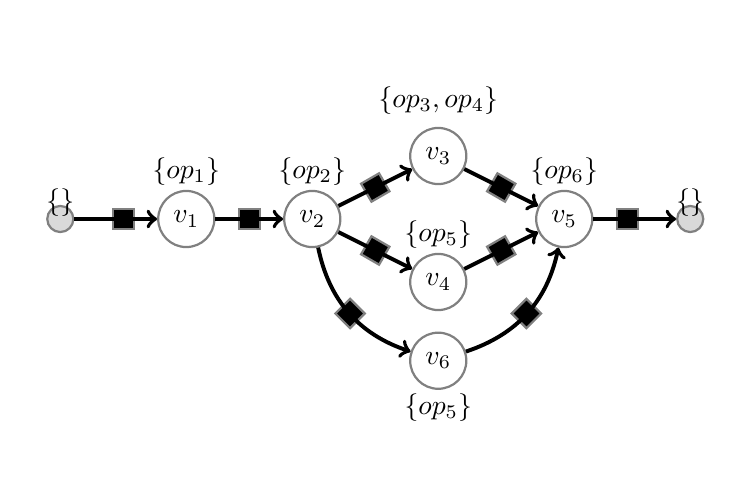
\begin{tikzpicture} 
 %[scale=.8,auto=left,every node/.style={circle,fill=blue!20}]
             [scale=.8,auto=left,every node/.style={circle,draw=black!50, thick},every path/.style={line width=0.5mm}]
 			\node[circle, fill=gray!30,label={[xshift=0cm, yshift=-0.4cm]$\{\optop\}$}] (v_t) at (-5,0) {$\verttop$};
             \node[label={[xshift=0cm, yshift=-0.4cm]$\{op_1\}$}] (v_1) at (-3,0) {$v_1$};
             \node[label={[xshift=0cm, yshift=-0.4cm]$\{op_2\}$}] (v_2) at (-1,0) {$v_2$};
             \node[label={[xshift=0cm, yshift=-0.6cm]$\{op_3,op_4\}$}] (v_3) at (1,1) {$v_3$};
             \node[label={[xshift=0cm, yshift=-0.4cm]$\{op_5\}$}] (v_4) at (1,-1) {$v_4$};
             \node[label={[xshift=0cm, yshift=-0.4cm]$\{op_6\}$}] (v_5) at (3,0) {$v_5$};  
             \node[label={[xshift=0cm, yshift=-1.6cm]$\{op_5\}$}] (v_6) at (1,-2.25) {$v_6$};                          
 			\node[circle, fill=gray!30,label={[xshift=0cm, yshift=-0.4cm]$\{\opbot\}$}] (v_b) at (5,0) {$\vertbot$};

			\node[rectangle,fill=black,minimum size=7.5pt] (v_c) at (-4,0) {};			
			\node[rectangle,fill=black,minimum size=7.5pt] (v_c) at (-2,0) {};
			\node[rectangle,fill=black,minimum size=7.5pt,rotate=30] (v_c) at (0,0.5) {};             
			\node[rectangle,fill=black,minimum size=7.5pt,rotate=60] (v_c) at (0,-0.5) {};          
			\node[rectangle,fill=black,minimum size=7.5pt,rotate=60] (v_c) at (2,0.5) {};  
			\node[rectangle,fill=black,minimum size=7.5pt,rotate=30] (v_c) at (2,-0.5) {}; 
			\node[rectangle,fill=black,minimum size=7.5pt] (v_c) at (4,0) {}; 	
			\node[rectangle,fill=black,minimum size=7.5pt] (v_c) at (-2,0) {};  
			\node[rectangle,fill=black,minimum size=7.5pt,rotate=45] (v_c) at (-0.4,-1.5) {};
			\node[rectangle,fill=black,minimum size=7.5pt,rotate=45] (v_c) at (2.4,-1.5) {};			
			
 			\path (v_t) edge[->] (v_1);
 			\path (v_1) edge[->] (v_2);
 			\path (v_2) edge[->] (v_3);
 			\path (v_2) edge[->] (v_4); 
 			\path (v_3) edge[->] (v_5); 						
 			\path (v_4) edge[->] (v_5);
 			\path (v_5) edge[->] (v_b);
 			
 			\path[]
            	(v_2) edge[->,bend right] (v_6)
                (v_6) edge[->,bend right] (v_5);
 		\end{tikzpicture}
	 	}
 	\end{center}
\caption{The graph for the plant introduced in Section~\ref{subsec:linear_model} with an additional cell, $v_6$, added.}
\label{fig:linear_plant_plus_graph}
\end{figure}


The plant with $v_6$ is then fed into the simulator for the experiment.
We keep the set of requirements and other configurations the same as the previous case for comparison.
The results are shown in Figure~\ref{fig:linear_plus_exp}.%Figures~\ref{fig:linear_plus_jph}, \ref{fig:linear_plus_total_widgets} and \ref{fig:linear_plus_end_to_end}.


From the simulation, we can observe that the throughput for all three requirements increases since the original bottleneck is removed after adding additional supports for $op_5$.
As a result, the end-to-end time for $R_2$ (\ie the requirement that requires $op_5$) decreases significantly.
Also, the total alive widgets slightly grow in this case because the capacity (\ie additional space for widgets to sit in) of the plant increases when the additional cell is added.
It's worth noting that $v_3$ becomes the new bottleneck in this setup as its support for $op_3$ has the highest time cost, which causes the congestion on the route to it.
